\chapter{Detalles de Implementación}\label{chapter:implementation}

%##1

Los modelos en build tienen que hacer todo el proceso de procesamiento de los datos, llenando tomados
las variables y estructuras que son necesarias para generar el texto en cada una de las etapas. Luego
en generate los modelos van en base a la representación interna de los datos, generando el texto de 
caa una de las piezas comunicativas.







%##2

Para poder trabajar más fácil con la propuesta, se proporcionó una interfaz gáfica. Esta interfaz es sencilla
 y se concibió utilizando el framework de python streamlit. Se da la opción a los usuarios de aportar
 datos en forma de archivos, ya sea a partir de definir la ruta local o cargando directamente el archivo.

 Para permitir  esta interacción se concibió una estructura intermedia para poder representar las tuplas
 de entrada en base a archivos json.  Cada tupla se concibe de la forma "id"

 donde cada valor representa el valor de la tupla............. en esa posición. Si no se proporciona uno de los 
 valores, esa posición se considera vacía. Ejemplo de representación se puede ver en imagen.

 Desde la primera interfaz se puede interactuar con el conjunto de datos de prueba que se concibieron
junto a la propuesta. Para ello hay que seleccionar el deporte deseado y uno entre los eventos de prueba.
El sistema mostrará el texto producido en pantalla, luego de presionar el botón "generar".


 




%##3

Para el llenado de la plantilla se utiliza la función select template, que a su vez emplea la función
fille template  y genre desambiguation.

La función  select template recibe el conjunto de posibles plantillas a emplear en la situación así como un 
diccionario de representación, donde las llaves constituyen las ranuras en las plantillas y los valores, el Valor
de ese dato en el contexto.

Como el sistema propuesto presenta cierto grado de sensibilidad ante la ausencia de datos, es posible
que haya plantillas en el conjunto para la que alguna de sus ranuras no tiene valor. Para esto, el algoritmo
selecciona automáticamente una plantilla del conjunto, si en el diccionario todas las ranuras tienen un valor 
correspondiente se selecciona, si no, se descarta y se repite el proceso. Siempre se garantiza que habrá
al menos una plantilla en el conjunto que funcione, porque presentará el subconjunto minimal de datos que
admite el sistema en ese contexto. La plantilla seleccionada se rellena utilizando el  método fill template
que sustituye las ranuras de la plantilla por el valor real.




\begin{figure}[!]
    \begin{center}
        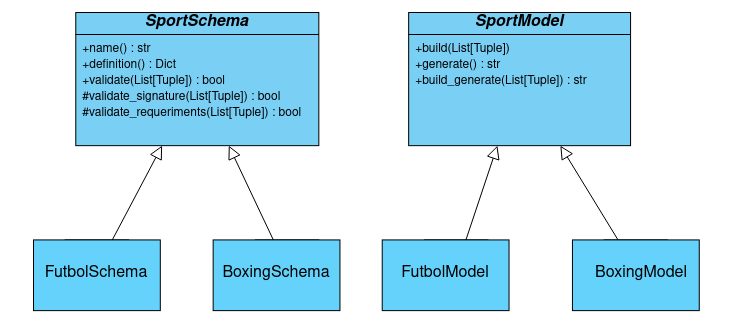
\includegraphics[width=\textwidth]{Graphics/classDef3.png}
    \end{center}
    \caption{Definición de las clases principales}
    \label{fig_classDef}
\end{figure}